\documentclass[../Article_Model_Parameters.tex]{subfiles}
\graphicspath{{\subfix{../Figures/}}}
\begin{document}
	
	%{\color{brown}Intro about extraction}\\
	The extraction of natural substances from solid materials and liquids with solvents have been a popular subject of research and development in the last years. Supercritical fluids have multiple applications in an extraction process due to the pressure-dependent dissolving power and both gas-and liquid-like properties (for example fluid-like density and gas-like diffusivity). Among different supercritical fluids, the supercritical $CO_2$ is one of the most popular due to it is nontoxic, non-flammable and non-corrosive properties. The critical point of $CO_2$ is relatively low ($73.8$ bar and $31 ^\circ C$), compare to other fluids. The supercritical extraction with $CO_2$ become attractive alternative, to replace traditional extraction techniques.
	
	%{\color{brown} Literature review of the models}\\
	The extraction of valuable compounds from fixed bed of biomass can be described by one of many mathematical models as presented by \citet{Huang2012}. The selection the extraction model is not arbitrary and should be based on the knowledge of phenomenons occurring in the operational unit. Each model has its own assumptions and describe different mass transfer mechanisms and equilibrium relationships. 
	
	Based on analogy to heat transfer, \citet{Reverchon1993} suggested a hot ball model, where the extraction process is treated analogously to a process in which a hot ball is cooled in a uniform medium. The hot ball model is used to describe an extraction process from solid particles which contains small quantities of solute so that the solubility is not a limiting factor. 
	
	\citet{Sovova1994} presented the Broken-and-Intact Cell model. The BIC model describes a system where the outer surfaces of particles have been mechanically interrupted. The solute from the broken cells is easily accessible for the solvent. The extraction of easily accessible solute is fast and directly controlled by its diffusion and convection in the solvent. However, the rest of the solute is less accessible because it is closed in the particle's core or intact cells. This solute slowly diffuses through the walls of a cell due to high mass transfer resistance.

    \citet{Reverchon1996} developed a model, which considers an oil as a single component and assumes that the extraction process is controlled by internal-mass transfer resistance. As a result of these assumptions, the external mass transfer was neglected. The original model of Reverchon does not consider the influence of axial dispersion and does not take into account the change of density and flow rate along the bed. 

    \iffalse
 
    In this model, the extraction process is divided into three periods controlled by different mass transfer mechanisms: Constant extraction rate (CER) period, Falling extraction rate (FER) period and Diffusion-controlled (DC) period.
	
	%{\color{brown}Methodology: sensitivity analysis }\\
	As in many engineering problems, mathematical modelling is crucial to mimic real-life objects, but it requires knowing multiple parameter values. One way to better understand the phenomena occurring in the process is to investigate the influences of various parameters on the model's output. One of the methods that can be applied is sensitivity analysis. Among different types of sensitivity analyses, there are two main groups: a local and global sensitivity analysis.
	The local method involves taking the total derivative of the output with respect to an input parameter at a single point. The derivative can be estimated directly by the automatic differentiation. {\color{blue}The total derivatives form an additional set of equations that is solved simultaneously with the original system. An alternative approach to the direct method is the Adjoint Sensitivity Analysis method. In this method, the original model is integrated to obtain the full trajectory of the state. Then the adjoint equation is solved backwards in time. The adjoint operates backwards in the sense that it determines a gradient with respect to input from a gradient with respect to output as discussed by \citet{Errico1997}.}
	The adjoint method is faster and requires the least memory than the local method. However, not all ODEs are stable under backwards integration. Moreover, both methods belong to one-at-a-time (OAT) methods, as they allow an investigation of the influence of only one parameter at a time. One way to determine the model response to "interactions" between parameters and to observe the non-linear behaviour of the system is to use higher-order derivatives.
	An alternative method is to apply a global sensitivity analysis, which utilises information about parameter uncertainty. A sensitivity analysis is considered global when all the parameters vary simultaneously. According to \citet{Razavi2015}, the main problem of generalising local sensitivity measures to represent "global" properties is the lack of a unique definition of global sensitivity. 
	\sout{These methods allow selecting the most influential parameters, which can be used for optimisation (the finding is a set of control variables, which requires the least effort to affect a model's output), model reduction (removing the least influential parameters), or parameter fitting. In this work, the example of supercritical extraction is used to show the practical application of sensitivity analysis. Some researchers working with the supercritical fluids extraction process examined the influence of the parameters on the model's output. Most of them perform a parametrisation of the process model and solve it multiple times for different combinations of parameters. The literature review is presented below.}
	{\color{blue}A sensitivity analysis is helpful to identify parameters that have the greatest effect on the model's output. The sensitivity analysis results can be used to find regions in the space of input factors for which the model output is maximum. Another application is model reduction - for example, by identifying and removing redundant parts of the model structure. In the case of parameter fitting with a large number of parameters, non-sensitive parameters can be excluded from the fitting procedure, reducing the computational cost. A sensitivity analysis is used to increase understanding of the relationships between input and output variables in a model.
		
		%{\color{brown} Literature review of the sensitivity analysis}\\
		\citet{Fiori_2007} presented how a model uncertainty affects a supercritical extraction process. Authors performed a local sensitivity analysis taken at the mean values of the parameters, determined during the parameter estimation. Their analysis shows the importance of two parameters: the particle diameter and the internal mass transfer coefficient. The authors found that the supercritical extraction process is almost completely insensitive during the first phase of the process (controlled by the solute's solubility in the supercritical solvent) for a change of these parameters. However, the authors claim that the model's sensitivity to parameters becomes high during the second phase of the process (controlled by internal diffusion).
		
		\citet{Rabi_2019} analysed how the different parameters affect the model's output. The parameters are dimensionless numbers (e.g., mass transfer Biot, Péclet and Damköhler numbers), which are assumed to take one of few discrete values. The simulations are performed for each value of parameters and compared with each other. The authors found that the Péclet number can strongly affect the extraction efficiency, so the diffusive transport should not be neglected. The authors investigated effect of the Damköhler number on the process. The authors observed that higher intra-particle diffusion accelerated solid particles depletion so that an optimal extraction time can then be looked for. Furthermore, the authors proved that others investigated parameters like partition coefficient and bed porosity influence the extraction yield. 
		
		\citet{Glover2008} presented a local sensitivity analysis for an adsorption process. Considering the similarities between extraction and adsorption processes, it is interesting to see how the same technique can be applied to different cases. The authors examine the sensitivity of the breakthrough of adsorption beds to system parameters. The impact of mass and energy transfer effects and adsorbent layer thicknesses are determined by calculating the derivatives of the outlet concentration and outlet temperature. The authors applied a Newton-based method along with the sensitivities to determine the optimal layering of an adsorption bed.}

    \fi
	
	In our model, the extraction process is assumed to operate in a semi-continuous mode in a cylindrical vessel. The solvent is firstly brought to super-critical condition, pumped through a fixed-bed, of finely chopped biomass, where the solute is extracted from the biomass. Then, the solvent and solute from the extractor are separated in a flush drum, and the extract is collected. The flow rate ($F_{in}$) and inlet temperature ($T_{in}$) of the extractor’s feed can be measured and manipulated. The pressure ($P$) in the vessel can be measured and manipulated, while the outlet temperature ($T_{out}$) can only be measured. A simplified flow diagram is depicted in Figure \ref{fig: SFE_drawing} .

    \begin{figure}[h!]
        \centering
        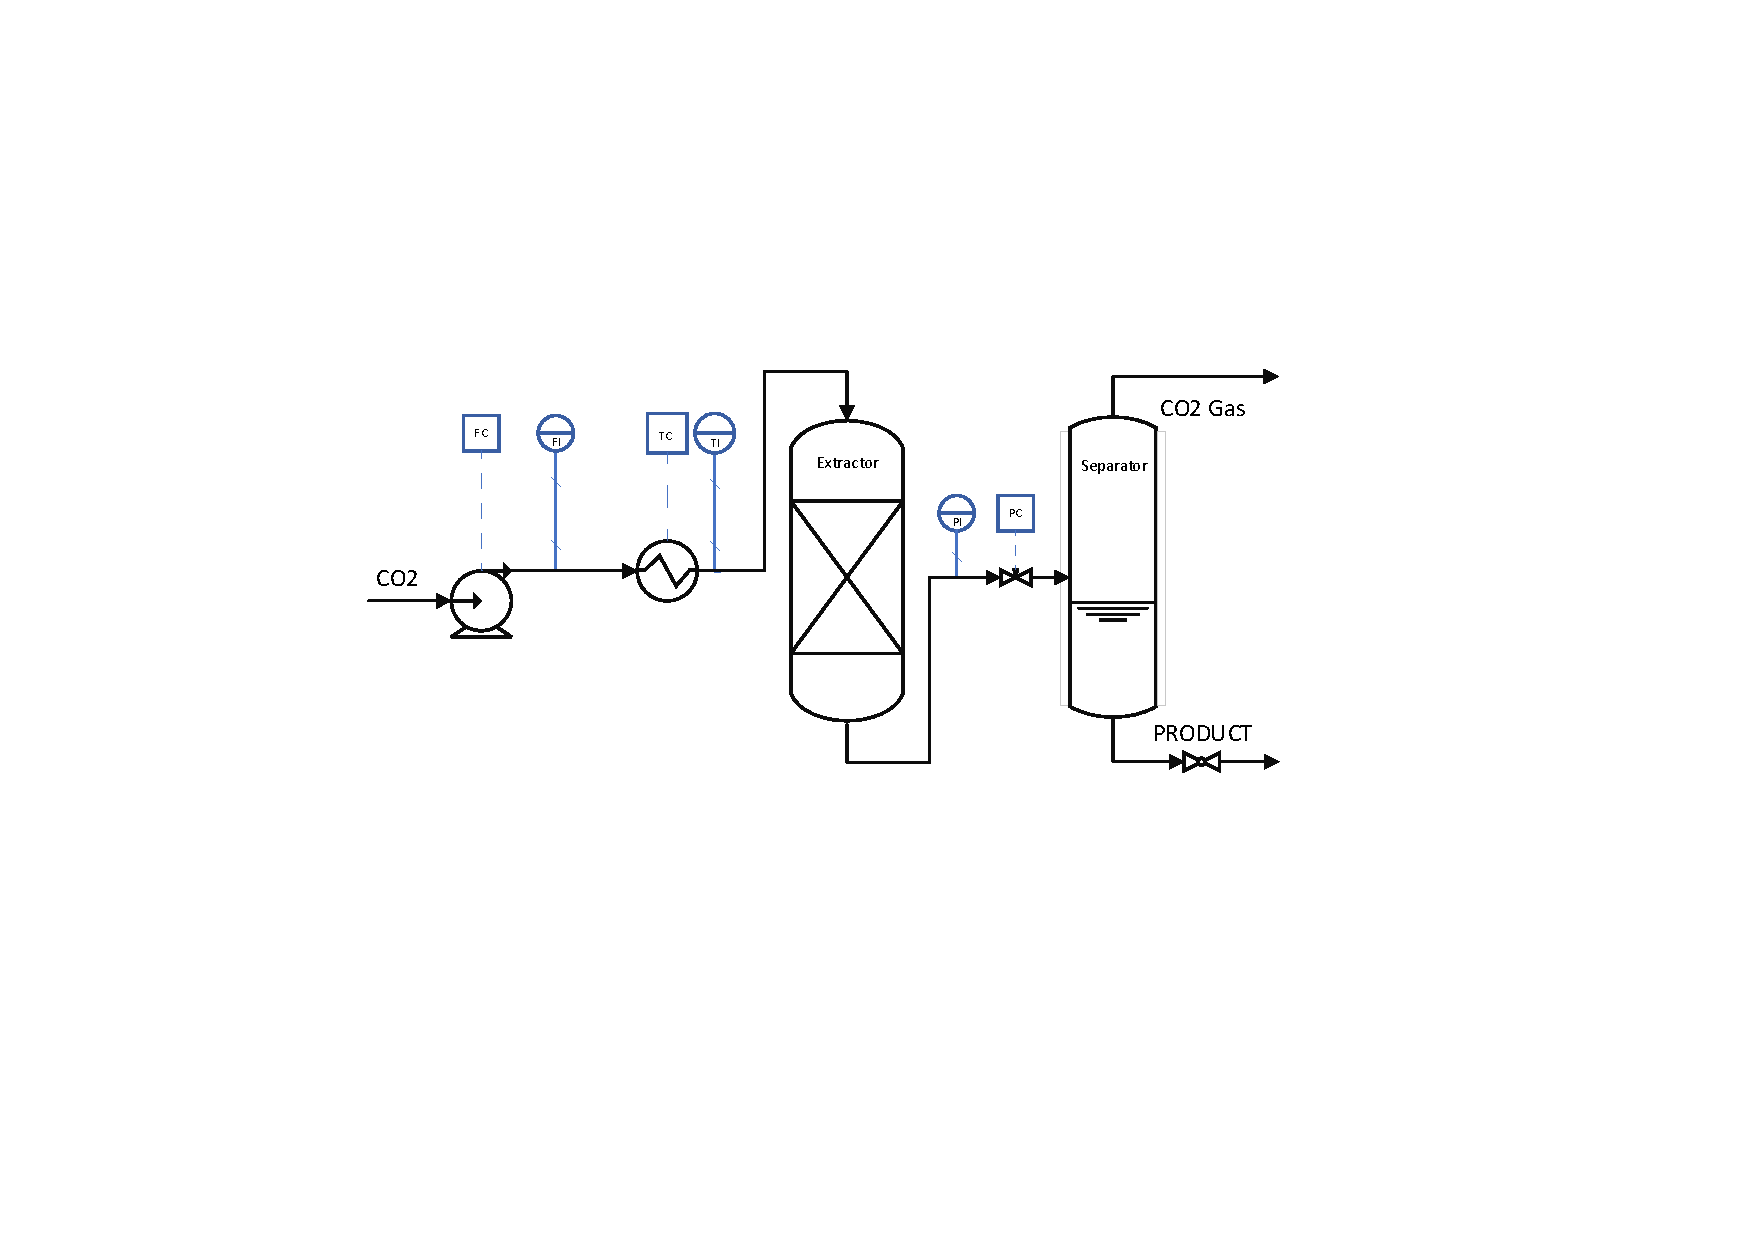
\includegraphics[width=0.95\columnwidth]{Figures/SFE_PFD_cropped.pdf}
        \caption{Process flow diagram ({\color{red}Font size}) }
        \label{fig: SFE_drawing}
    \end{figure}
	
\end{document}